% !TEX TS-program = pdflatex
% !TEX encoding = UTF-8 Unicode

\documentclass[specialist,
               substylefile = spbu.rtx,
               subf, 
               %href,
               colorlinks=true, 12pt]{disser}

\usepackage[
  a4paper, mag=1000, includefoot,
  left=3cm, right=1.5cm, top=2cm, bottom=2cm
, headsep=1cm, footskip=1cm]
{geometry}

\usepackage[utf8]{inputenc} % set input encoding (not needed with XeLaTeX)
\usepackage[T2A]{fontenc}
\usepackage[russian]{babel}
\usepackage{indentfirst}
\usepackage{amsmath}
\usepackage{amsthm}
\usepackage{amssymb}
\usepackage{amsfonts}
\usepackage{graphicx}
\usepackage{xcolor}
\usepackage{wrapfig}
%\usepackage{subfigure}
\usepackage{longtable}
\usepackage{array}
\usepackage{hyperref}
\usepackage{caption}
\usepackage{subcaption}
\usepackage{float}

\usepackage{booktabs}
\usepackage{multirow}
\usepackage{rotating}

\usepackage{bm}

\newcommand{\specialcell}[2][c]{%
  \begin{tabular}[#1]{@{}c@{}}#2\end{tabular}}
  
\newcommand{\vect}[1]{\boldsymbol{\mathbf{#1}}}  
  
\newcommand{\T}{\mathrm{T}} 
\newcommand{\E}{\mbox{E}} 

\newtheorem{determination}{Определение}
\newtheorem{theorem}{Теорема}
\newtheorem{stat}{Утверждение}
\newtheorem{remark}{Замечание}
\newtheorem{corollary}{Следствие}

\newcolumntype{C}[1]{>{\centering}m{#1}}

\newcommand{\R}{\mathbb{R}}

\ifpdf\usepackage{epstopdf}\fi 
% Использовать полужирное начертание для векторов
\let\vec=\mathbf
% Включать подсекции в оглавление
\setcounter{tocdepth}{3}

\DeclareMathOperator*{\argmin}{argmin}
\DeclareMathOperator*{\argmax}{argmax}

\newtheorem{definition}{Определение}

\begin{document}

\institution{%
Санкт-Петербургский государственный университет \\
    Прикладная математика и информатика \\
    Статистическое моделирование
}

\title{Рукавишникова Анна\\ Страшко Владислав\\ Сандул Михаил}
\topic{\normalfont\scshape %
Глубокое обучение}
\author{}

\city{Санкт-Петербург}
\date{2019}

\maketitle
\tableofcontents

\newpage

\section{Глубокое обучение в парадигме методов машинного обучения}

Глубокое обучение --- это совокупность широкого семейства методов машинного обучения, основанных на имитации работы человеческого мозга, а именно, на взаимодействии нейронов. Термин <<глубокое обучения>> появился ещё в 1980-х, но до середины 2000-х для реализации методов глубокого обучения не хватало вычислительных мощностей существующих компьютеров. Стоит отметить, что часто под данным термином подразумеваются многослойные нейронные сети.


Существенное отличие глубокого обучения от машинного обучения как такового заключается в том, что часть, касаемая feature engineering (feature extraction) в классических методах машинного обучения решается вручную, а в глубоком обучении она решается (может решаться) автоматически.

\begin{figure}[!h]
\begin{center}
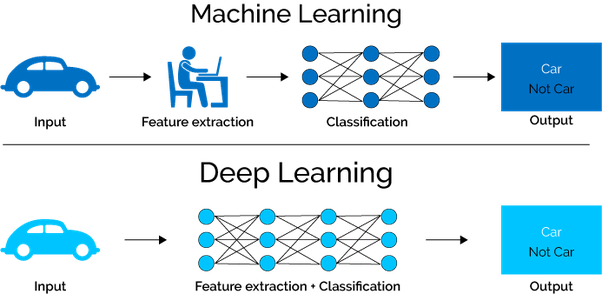
\includegraphics[width=0.7\linewidth]{MLvsDL}
\end{center}
\caption{Отличие между машинным обучением и глубоким обучением}
\end{figure}


Основными представителями алгоритмов глубокого обучения являются:
\begin{itemize}
\item свёрточные нейронные сети (CNN),
\item рекуррентные нейронные сети (RNN).
\end{itemize}

Свёрточные нейронные сети используются, как правило, для анализа изображений, текстов и речи, а рекуррентные --- для обработки объектов, характеризующихся наличием последовательной структуры. Например, рекуррентные нейронные сети часто используют для обработки текстов на естественном языке, обработки аудио и видео.

\section{Рекуррентные нейронные сети (RNN)}

В связ с тем, что свёрточным нейронным сетям был посвящён один из прошлых семинаров, сейчас поподробнее остановимся на рекуррентных нейронных сетях. 


Идея, заложенная в создание рекуррентных нейронных сетей состоит в желании имитации человеческой памяти. Иными словами, при обработке тех или иных объектов с последовательной структурой нам бы хотелось, чтобы нейронная сеть сохраняла информацию о своём предыдущем состоянии. Представим, например, что мы хотим классифицировать события, происходящие в фильме. Непонятно, как традиционная нейронная сеть могла бы использовать рассуждения о предыдущих событиях фильма, чтобы получить информацию о последующих. Решить эту проблемы помогают рекуррентные нейронные сети, благодаря тому, что они содержат обратные связи и позволяют сохранять информацию.

\subsection{Архитектура рекуррентной нейронной сети}

Рассмотрим устройство рекуррентных нейронных сетей. Пусть $x_t$ --- входной вектор в момент времени $t$, $h_t$ --- вектор скрытого состояния в момент времени $t$, $y_t$ --- выходной вектор в момент времени $t$. Стоит заметить, что  в некоторых приложениях $y_t \equiv h_t$. Таким образом, схема  рекуррентной нейронной сети может быть представлена следующим образом:

\begin{figure}[!h]
\begin{center}
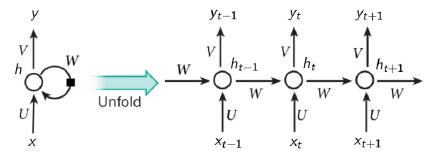
\includegraphics[width=0.7\linewidth]{rnn_1}
\end{center}
\caption{Схема рекуррентной нейронной сети с развёрткой обратной связи}
\end{figure}

На схеме выше слева обратная связь схематично обозначена стрелкой, выходящей из фрагмента (модуля)  сети со скрытым состоянием $h$ и входящей в  него же. Наличие такой обратной связи позволяет передавать информацию от одного шага сети к другому. $\mathbf{W}, \mathbf{U}$ и $\mathbf{V}$ --- это матрицы параметров, для которых справедливы следующие соотношения:
\begin{eqnarray*}
h_t &=& \sigma_h(\mathbf{U}x_t + \mathbf{W}h_{t-1}), \\
y_t &=& \sigma_y(\mathbf{V}h_t),
\end{eqnarray*}
где $\sigma_h$ и $\sigma_y$ --- функции активации.

Поясним разворачивание (unfolding) обратной связи  на примере работы рекуррентной нейронной сети с предложением, положив для определённости $t = 1$. В таком случае $x$ будет являться самим предложением, а $x_0$ будет первым словом в данном предложении. Это слово мы подаём на вход нейрону. Обработав его, нейрон выдаст значение $y_0$. Переходя к обработке следующего слова $x_1$, нейрон получит на вход не только само это слово, но и информацию, полученную от обработки первого слова этого предложения $x_0$. Тем самым, сеть сможет уловить некоторую взаимосвязь между первым и вторым словом в предложении. В качестве примера можно также рассмотреть временной ряд. В этом случае $x$ --- рассматриваемый временной ряд целиком, а $h$ --- его неизвестный сигнал. В то время как $x_t$ --- вектора вложения данного ряда (размера $1$).

\subsection{Обучение рекуррентной нейронной сети}

В процессе обучения рекуррентной сети стоит задача минимизации следующего функционала:

\begin{equation*}
\sum_{t=0}^{T} \mathcal{L}_t (\mathbf{U}, \mathbf{V}, \mathbf{W}) \rightarrow \min_{\mathbf{U},\mathbf{ V}, \mathbf{W}},
\end{equation*}
где $\mathcal{L}_t (\mathbf{U}, \mathbf{V}, \mathbf{W}) = \mathcal{L} (y_t(\mathbf{U}, \mathbf{V}, \mathbf{W}))$ --- потеря от предсказания $y_t$.


Также в отличие от обычных нейронных сетей (не рекуррентных) используется специальный вариант обратного распространения ошибок --- Backpropagation Through Time (BPTT):

\begin{equation*}
\dfrac{\partial \mathcal{L}_t}{\partial \mathbf{W}} = \dfrac{\partial \mathcal{L}_t}{\partial y_t} \dfrac{\partial y_t}{\partial h_t} \sum_{k=0}^t \left( \prod_{i = k + 1}^t \dfrac{\partial h_i}{\partial h_{i-1}} \right) \dfrac{\partial h_k}{\partial \mathbf{W}}.
\end{equation*}

Поскольку рекуррентная сеть получается очень глубокой, то становится острой проблема затухающего градиента. Это происходит засчёт того, что подсчитывая градиент в методе обратного распространения ошибки (backpropagation) при обновлении весов, переходя от одного скрытого слоя к другому, у нас появляется множитель в виде некоторой матрицы в очень большой степени. Элементы этой матрицы могут быть очень близки к нулю, тогда возводя эту матрицу в очень большую степень мы получим вырождение градиента с экспоненциальной скоростью в ноль (затухание). Существует и противоположная крайность такой проблемы, называемая, взрывом градиента. Одним из решений данной проблемы является ограничение частной производной: $\dfrac{\partial h_i}{\partial h_{i-1}} \rightarrow 1.$ Именно эта идея реализована в сетях долгой краткосрочной памяти (Long short-term memory, LSTM).

\section{Нейронные сети долгой краткосрочной памяти (LSTM)}

Мотивацией к созданию LSTM сетей послужило следующее соображение. Рекуррентные нейронные сети хорошо справились бы, например, со следующей задачей: мы хотели бы предсказать последнее слово в предложении <<облака плывут по небу>> на основании предыдущих. В таком случае для предсказания нам не нужен более широкий контекст, довольно очевидно из предыдущего контекста, что последним будет слово <<небо>>. То есть в таком примере, где дистанция между актуальной информацией и местом, где она понадобилась, невелика, рекуррентные нейронные сети могут обучиться, используя информацию из прошлого. Однако, можно столкнуться со случаем, когда необходимо больше контекста для предсказания последнего слова, как, например, в предложении <<Я много лет жил во Франции со своими родителями и старшими братьями, поэтому я бегло говорю по-французски>>. Ближайшие к последнему слову контекст предполагает, что последним словом будет название языка, но, чтобы установить, какого именно языка, нам необходимо помнить о слове <<Франции>> из более отдалённого контекста.


Таким образом,  известно, что по мере роста расстояния между актуальной информацией и точкой её применения, рекуррентные нейронные сети теряют способность находить смысловые связи. Эта проблема именуется проблемой долговременных зависимостей. Сети LSTM разработаны специально, чтобы избежать проблемы долговременной зависимости.

\subsection{Устройство LSTM сети}

Детально рассмотрим устройство и принцип работы сетей LSTM. Структура LSTM, как и для любой RNN сети, напоминает цепочку, состоящую из повторяющихся модулей. Однако, в отличие от рекуррентных сетей, где модуль состоит из одного слоя нейронов, LSTM сеть имеет уже четыре взаимодействующих между собой слоя. Ключевым состоянием LSTM сети является вектор состояния ячейки $C_t$ в момент времени $t$.

\begin{figure}[!h]
\begin{center}
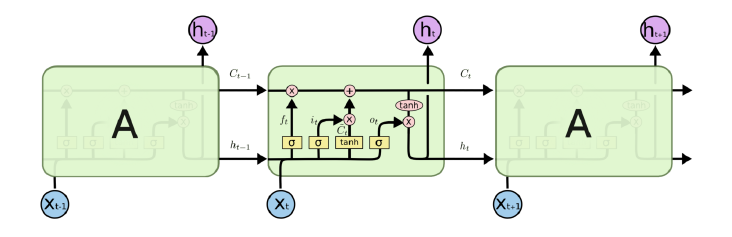
\includegraphics[width=0.85\linewidth]{lstm_KV}
\end{center}
\caption{Структура LSTM сети}
\end{figure}

\begin{figure}[!h]
\begin{center}
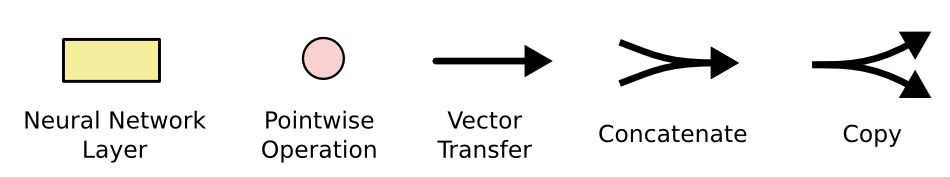
\includegraphics[width=0.7\linewidth]{lstm_signs}
\end{center}
\caption{Условные обозначения}
\end{figure}


Перейдём к пошаговому разбору алгоритма работы LSTM сети.

\begin{figure}[!h]
\begin{center}
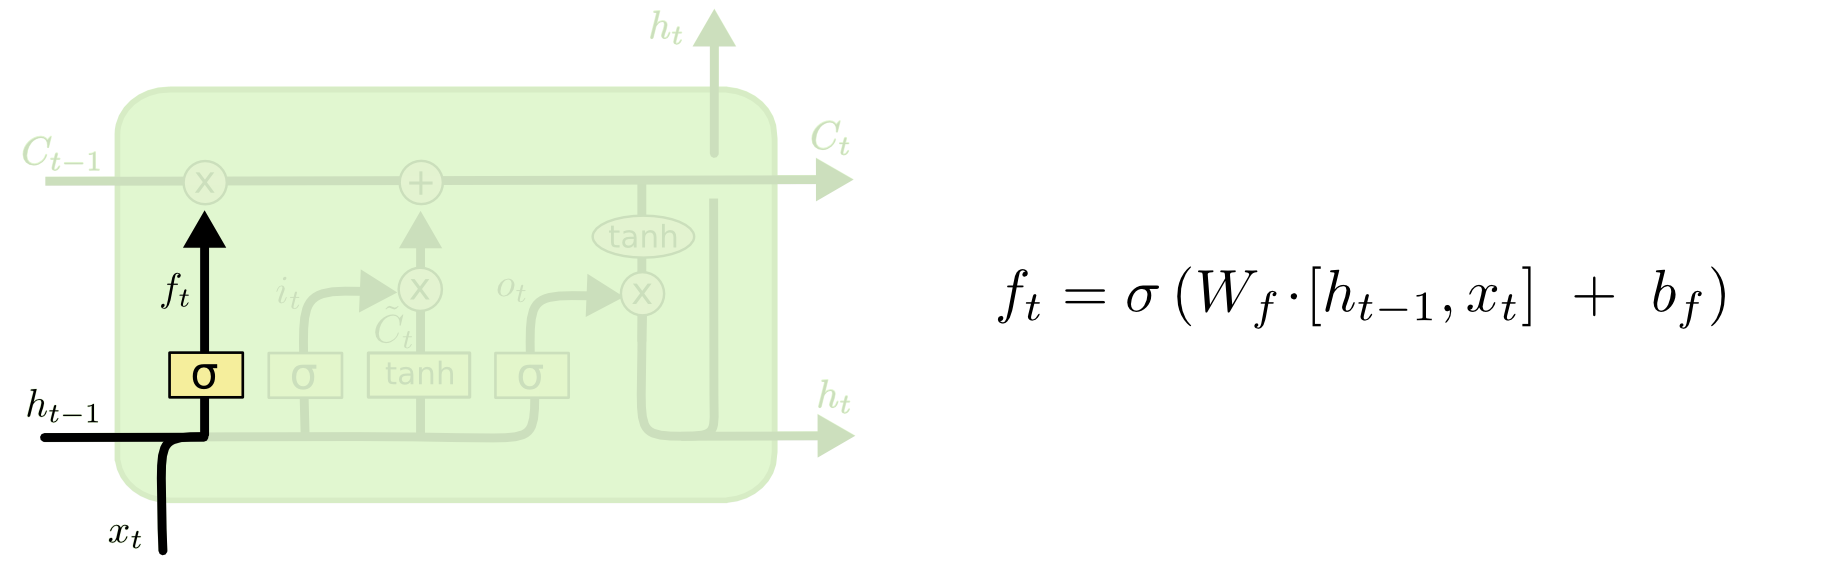
\includegraphics[width=0.55\linewidth]{lstm_forget_gate}
\end{center}
\caption{Слой фильтра забывания}
\end{figure}


Итак, на первом шаге первому слою LSTM ячейки в момент времени $t$ поступают на вход два значения: $h_{t-1}$ --- вектор скрытого состояния с предыдущего момента времени и $x_t$ --- входной вектор в момент времени $t$. Данный слой называется слоем фильтра забывания (forget gate layer), так как на этом шаге определяется, какие координаты вектора состояния $C_{t-1}$ нужно запомнить, а какие --- нет. Преобразование входных данных осуществляется следующим образом:

\begin{equation}
f_t = \sigma(\mathbf{W}_f \dot [h_{t-1},x_t] + b_f),
\label{eq:f_t}
\end{equation}
где $\sigma$ --- сигмоида, $\mathbf{W}_f$ и $b_f$ --- матрица и вектор параметров, соответственно, а операция $ [h_{t-1},x_t]$ означает конкатенацию двух векторов. 

\begin{figure}[!h]
\begin{center}
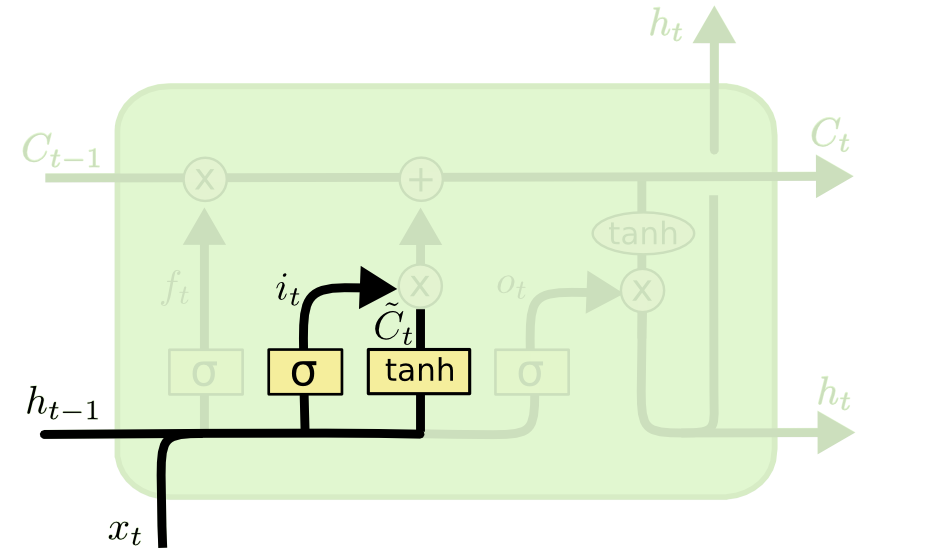
\includegraphics[width=0.55\linewidth]{lstm_layer_gate}
\end{center}
\caption{Слой входного фильтра и tanh-слой}
\end{figure}


На следующем шаге необходимо решить, какая новая информация будет храниться в состоянии ячейки. Данный шаг будет осуществляться в два этапа. Сначала слой фильтра входных данных (input gate layer) с параметрами $\mathbf{W}_i$, $b_i$ определяет, какие координаты вектора состояния нужно обновить:

\begin{equation}
i_t = \sigma(\mathbf{W}_i \cdot [h_{t-1},x_t] + b_i).
\label{eq:i_t}
\end{equation}


Затем tanh-слой с параметрами $\mathbf{W}_C$, $b_C$ строит вектор новых значений-кандидатов $\widetilde{C}_t$, которые можно добавить в состояние ячейки:

\begin{equation*}
\widetilde{C}_t = tanh(\mathbf{W}_C \cdot [h_{t-1},x_t] + b_C).
\end{equation*}

\begin{figure}[!h]
\begin{center}
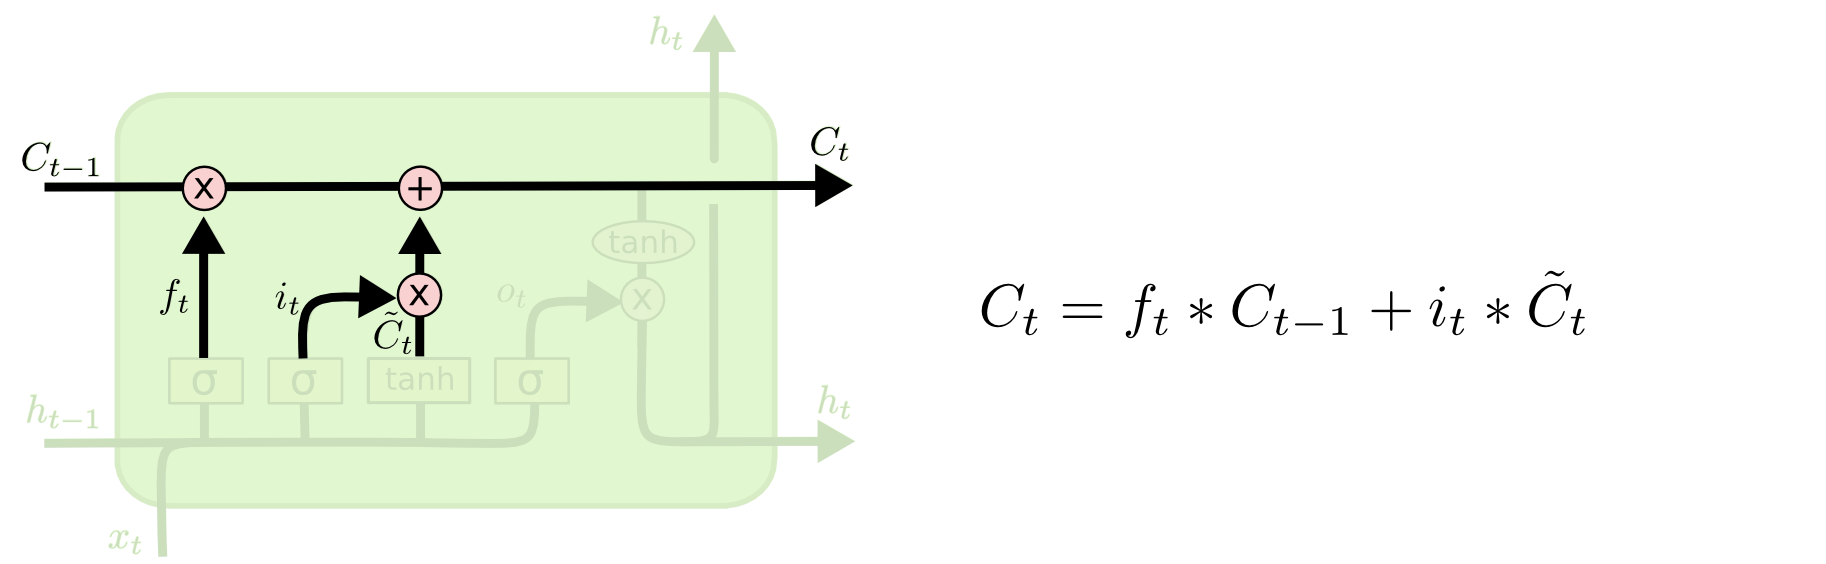
\includegraphics[width=0.55\linewidth]{lstm_state}
\end{center}
\caption{Обновление состояния ячейки}
\end{figure}


На третьем шаге новое состояние $C_t$  формируется как смесь старого состояния $C_{t-1}$ с фильтром $f_t$ и вектора значений-кандидатов $ \widetilde{C}_t$ с фильтром $i_t$ (используем покоординатное умножение):

\begin{equation*}
C_t = f_t\cdot C_{t-1} + i_t\cdot \widetilde{C}_t.
\end{equation*}

На этом шаге. очевидно, настраиваемых параметров нет, так как мы используем уже полученные ранее результаты.


Теперь осталось только решить, какую информацию мы хотим получить на выходе. Выходные данные будут основаны на нашем состоянии ячейки, к которому будут применены некоторые фильтры.

\begin{figure}[!h]
\begin{center}
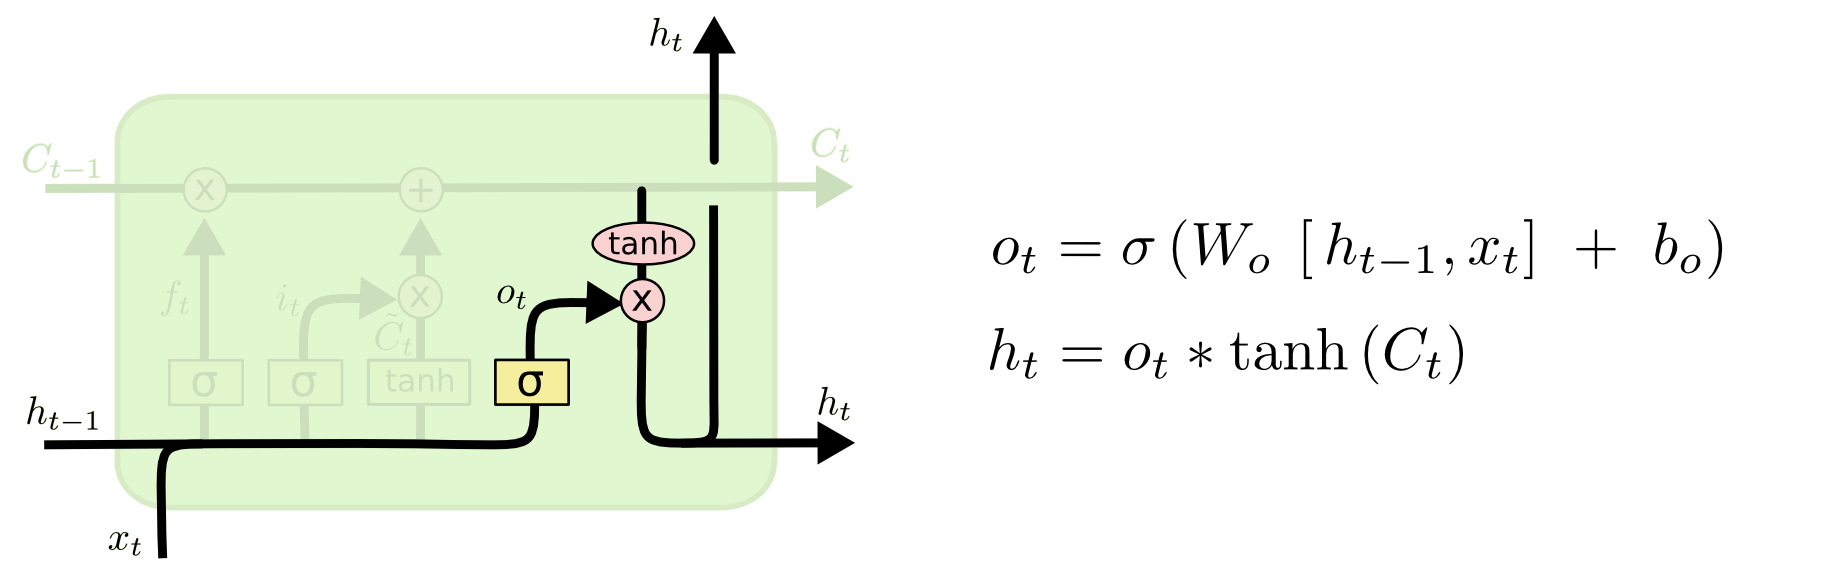
\includegraphics[width=0.55\linewidth]{lstm_out}
\end{center}
\caption{Обновление состояния ячейки}
\end{figure}


Сначала мы применяем фильтр выходных данных (output gate) с параметрами $\mathbf{W}_o$, $b_o$, который решает, какую информацию из состояния ячейки мы будем выводить, то есть какие координаты вектора состояния $C_t$ нужно выдать:

\begin{equation}
o_t = \sigma(\mathbf{W}_o[h_{t-1},x_t] + b_o).
\label{eq:o_t}
\end{equation}


Затем значения состояния ячейки проходят через tanh-слой, чтобы получить на выходе значения из диапазона от $-1$ до $1$ в качестве выходного сигнала $h_t$, и перемножаются с выходными значениями $o_t$, что позволяет выводить только требуемую информацию:


\begin{equation*}
h_t = o_t \cdot tanh(C_t).
\end{equation*}


\subsection{Вариации LSTM}

Существует множество различных вариаций LSTM сетей. Отличие между ними незначительны, однако, о некоторых из них стоит упомянуть. 


Одна из популярных вариаций LSTM, предложенная Герсом и Шмидхубером в работе \cite{peephole}, характеризуется добавлением так называемых <<смотровых глазков>> или <<замочных скважин>> (peephole connections). С их помощью слои фильтров могут видеть состояние ячейки.

\begin{figure}[!h]
\begin{center}
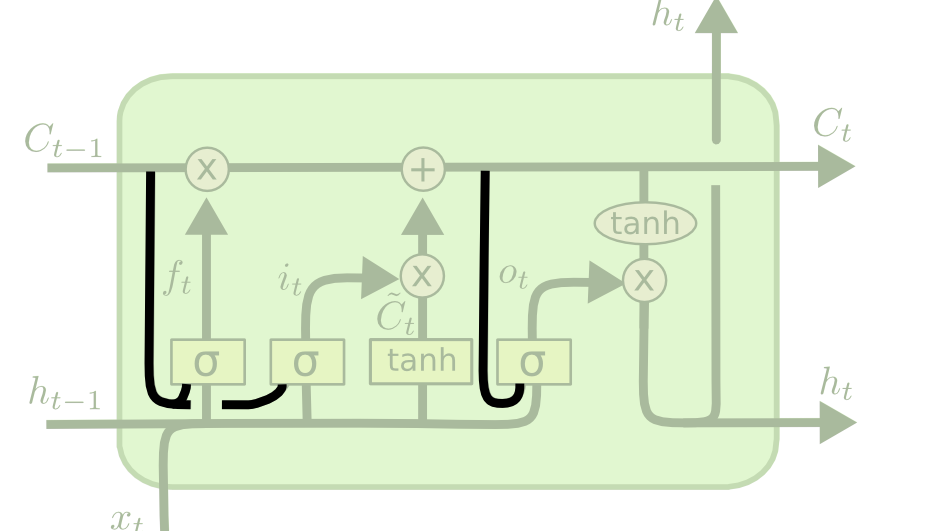
\includegraphics[width=0.55\linewidth]{lstm_peepholes}
\end{center}
\caption{LSTM c ``замочными скважинами''}
\end{figure}


На схеме выше <<замочные скважины'>> есть у каждого слоя, но в некоторых случаях они добавляются лишь к некоторым слоям. В такой вариации LSTM число параметров модели увеличивается, а, кроме того, формулы \eqref{eq:f_t}, \eqref{eq:i_t} и \eqref{eq:o_t} видоизменяются следующим образом:

\begin{eqnarray*}
f_t &=& \sigma(\mathbf{W}_f \cdot [C_{t-1},h_{t-1},x_t] + b_f), \\
i_t &=& \sigma(\mathbf{W}_i \cdot [C_{t-1},h_{t-1},x_t] + b_i), \\
o_t &=& \sigma(\mathbf{W}_o \cdot[C_t,h_{t-1},x_t] + b_o).
\end{eqnarray*}


Немного больше от стандартных LSTM сетей отличается следующая модификация --- управляемые рекуррентные нейроны (блоки) (Gated Recurrent Unit, GRU). Впервые эта вариация LSTM была описана в работе \cite{cho}. Важной особенностью данной нейронной сети является объединение фильтра забывания (forget gate)  и входа (input gate) в один фильтр обновления (update gate). Кроме того, состояние ячейки $C_t$ объединяется со скрытым состоянием $h_t$. Построенная в результате модель проще, чем стандартная LSTM (она имеет меньше параметров), и популярность ее неуклонно возрастает.

\begin{figure}[!h]
\begin{center}
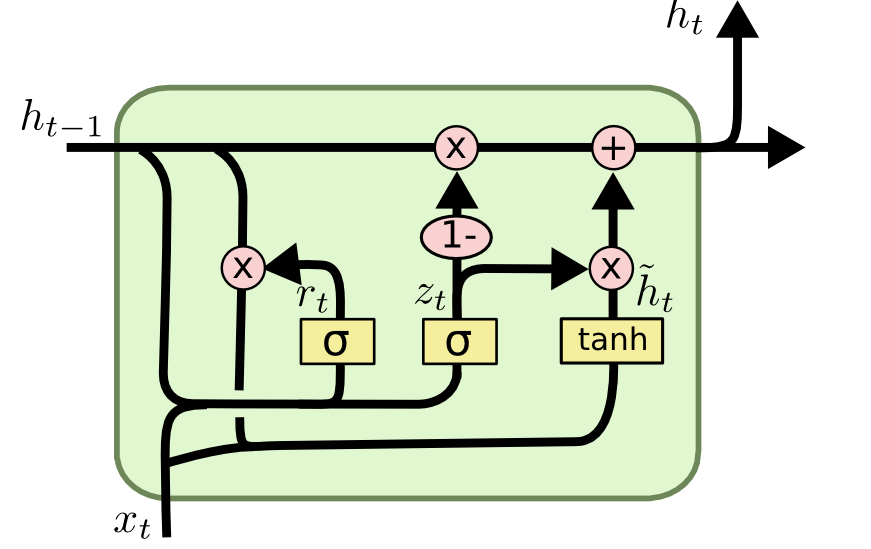
\includegraphics[width=0.55\linewidth]{lstm_gru}
\end{center}
\caption{LSTM: Gated Recurrent Unit (GRU)}
\end{figure}


Действия фильтров в GRU сети описываются следующими уравнениями:

\begin{eqnarray*}
z_t &=& \sigma(\mathbf{W}_z \cdot [h_{t-1},x_t]), \\
r_t &=& \sigma(\mathbf{W}_r \cdot [h_{t-1},x_t]), \\
\widetilde{h}_t &=& tanh(\mathbf{W} \cdot[r_t \cdot h_{t-1},x_t]), \\
h_t &=& (1 - z_t) \cdot h_{t-1} + z_t \cdot \widetilde{h}_t. 
\end{eqnarray*}
 

Существует множество других модификаций LSTM сетей, как, например, глубокие управляемые рекуррентные нейронные сети (Depth Gated RNNs), представленные в работе \cite{yao}. Сравнение самых популярных вариаций LSTM представлено в работе \cite{Jozefowicz}, авторы которой приходят к выводу о том, что все модификации приблизительно одинаковы.

\section{Применение RNN к временным рядам}

Одной из задач, для которых используются рекуррентные нейронные сети, является задача предсказания временных радов. В таком случае на вход рекуррентной нейронной сети подаются отдельно точки временного ряда, и для обработки используется архитектура RNN сетей, называемая one to many.

\begin{figure}[!h]
\begin{center}
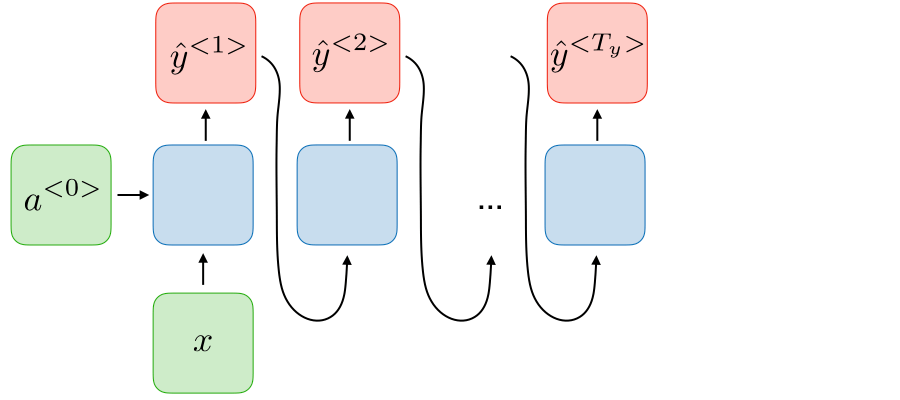
\includegraphics[width=0.55\linewidth]{rnn-one-to-many}
\end{center}
\caption{RNN: архитектура one to many}
\end{figure}

Здесь $x$ --- последняя точка временного ряда, $a^{<0>}$ --- скрытое состояние сети, полученное на предыдущем шаге (в прошлый момент времени), и мы строим прогноз на $T_y$ точек вперёд. Для получения каждого следующего прогноза мы используем полученное предсказание на предыдущем шаге. Если бы мы хотели сделать прогноз только на одну точку вперёд, то, как частный случай, мы бы использовали структуру one to one.

\bibliographystyle{gost2008}
\bibliography{deep_learning}

\end{document}
